%%%%%%%%%%%%%%%%%%%%%%%%%%%%%%%%%%%%%%%%%
% Beamer Presentation
% LaTeX Template
% Version 1.0 (10/11/12)
%
% This template has been downloaded from:
% http://www.LaTeXTemplates.com
%
% License:
% CC BY-NC-SA 3.0 (http://creativecommons.org/licenses/by-nc-sa/3.0/)
%
%%%%%%%%%%%%%%%%%%%%%%%%%%%%%%%%%%%%%%%%%

%----------------------------------------------------------------------------------------
%	PACKAGES AND THEMES
%---------------------------------------------------------------------------------------

\documentclass{beamer}
\usepackage[spanish]{babel}
 \usepackage{algpseudocode}
\usepackage[utf8]{inputenc}
\mode<presentation> {

% The Beamer class comes with a number of default slide themes
% which change the colors and layouts of slides. Below this is a list
% of all the themes, uncomment each in turn to see what they look like.

%\usetheme{default}
%\usetheme{AnnArbor}
%\usetheme{Antibes}
%\usetheme{Bergen}
%\usetheme{Berkeley}
%\usetheme{Berlin}
%\usetheme{Boadilla}
%\usetheme{CambridgeUS}
%\usetheme{Copenhagen}
%\usetheme{Darmstadt}
%\usetheme{Dresden}
%\usetheme{Frankfurt}
%\usetheme{Goettingen}
%\usetheme{Hannover}
%\usetheme{Ilmenau}
%\usetheme{JuanLesPins}
%\usetheme{Luebeck}
%\usetheme{Madrid}
%\usetheme{Malmoe}
%\usetheme{Marburg}
%\usetheme{Montpellier}
\usetheme{PaloAlto}
%\usetheme{Pittsburgh}
%\usetheme{Rochester}
%\usetheme{Singapore}
%\usetheme{Szeged}
%\usetheme{Warsaw}

% As well as themes, the Beamer class has a number of color themes
% for any slide theme. Uncomment each of these in turn to see how it
% changes the colors of your current slide theme.

%\usecolortheme{albatross}
%\usecolortheme{beaver}
%\usecolortheme{beetle}
%\usecolortheme{crane}
%\usecolortheme{dolphin}
%\usecolortheme{dove}
%\usecolortheme{fly}
%\usecolortheme{lily}
%\usecolortheme{orchid}
%\usecolortheme{rose}
%\usecolortheme{seagull}
%\usecolortheme{seahorse}
%\usecolortheme{whale}
%\usecolortheme{wolverine}

%\setbeamertemplate{footline} % To remove the footer line in all slides uncomment this line
%\setbeamertemplate{footline}[page number] % To replace the footer line in all slides with a simple slide count uncomment this line

%\setbeamertemplate{navigation symbols}{} % To remove the navigation symbols from the bottom of all slides uncomment this line
}

\usepackage{graphicx} % Allows including images
\usepackage{booktabs} % Allows the use of \toprule, \midrule and \bottomrule in tables

%----------------------------------------------------------------------------------------
%	TITLE PAGE
%----------------------------------------------------------------------------------------

\title[Practica 1]{Práctica 2: Divide y vencerás} % The short title appears at the bottom of every slide, the full title is only on the title page

\author{Algorítmica} % Your name
\institute[UGR] % Your institution as it will appear on the bottom of every slide, may be shorthand to save space
{
Universidad de Granada \\ % Your institution for the title page
\medskip

}
\date{\today} % Date, can be changed to a custom date

\begin{document}

\begin{frame}
\titlepage % Print the title page as the first slide
\end{frame}

\begin{frame}
\frametitle{Índice} % Table of contents slide, comment this block out to remove it
\tableofcontents % Throughout your presentation, if you choose to use \section{} and \subsection{} commands, these will automatically be printed on this slide as an overview of your presentation
\end{frame}

%----------------------------------------------------------------------------------------
%	PRESENTATION SLIDES
%----------------------------------------------------------------------------------------

\section{Introducción }
\begin{frame}
	\frametitle{Introducción}
	\begin{itemize}
		\item El objetivo de ésta práctica era resolver uno de los cinco problemas dados aplicando la técnica divide y vencerás.
		\item Además de la elaboración del programa, hemos calculado las distintas eficiencias, comparándolo también con un algoritmo de ordenación por fuerza bruta.
		\item Para medir tiempos hemos utilizado la biblioteca de C++ más moderna y precisa destinado a obtener tiempos de reloj: la biblioteca \textbf{chrono}
	
	\end{itemize}
\end{frame}


%------------------------------------------------
\section{Ejercicio} % Sections can be created in order to organize your presentation into discrete blocks, all sections and subsections are automatically printed in the table of contents as an overview of the talk
%------------------------------------------------
\begin{frame}
	\frametitle{Enunciado del ejercicio}
	Dados K vectores de longitud N ordenado cada uno de ellos obtener un tamaño de N*K ordenado.
\end{frame}

%------------------------------------------------
\section{Fuerza bruta} % Sections can be created in order to organize your presentation into discrete blocks, all sections and subsections are automatically printed in the table of contents as an overview of the talk
%------------------------------------------------
\begin{frame}
	\frametitle{Pseudocódigo}
    
    Algoritmo Fuerza bruta.
	\begin{algorithmic}
	\Require Vectores ordenados, numero de estos y tamaño
	
 	\State{V1 = V[0]}
 	\State{Vfinal = V[1]}
 	\State{Vfinal = OrdenarVectores(V1,Vfinal)}
	\For {i=2 hasta i=k-1 }
 	   \State{V1=V[i]; }
 	   \State{Vfinal= OrdenarVectores(V1,Vfinal);}
  	   \State{i++;}
	\EndFor
	\end{algorithmic}	
	
\end{frame}

\begin{frame}
	\frametitle{Eficiencia}

	\begin{figure}[H]
\centering
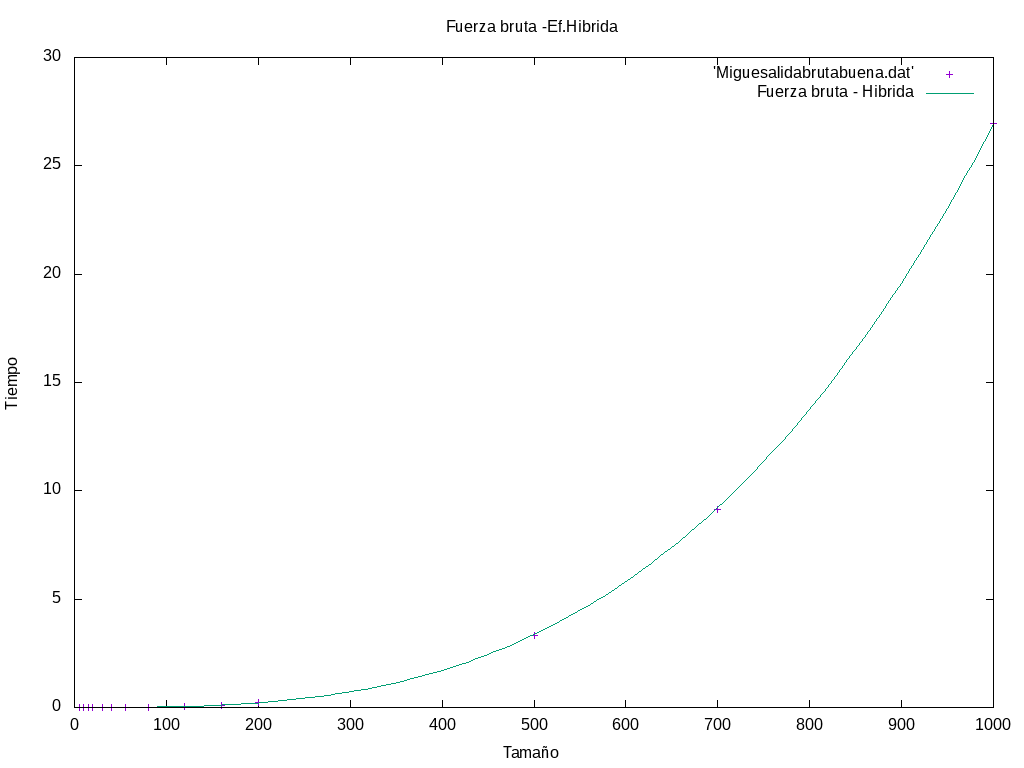
\includegraphics[width=0.7\linewidth]{../salidas-algoritmos/fuerzabruta-hibrida}
\caption{La eficiencia resultante es de n cubo}
\label{fig:fuerzabruta-hibrida}
\end{figure}
	
\end{frame}

\section{Algoritmo DyV} % Sections can be created in order to organize your presentation into discrete blocks, all sections and subsections are automatically printed in the table of contents as an overview of the talk
%------------------------------------------------
\begin{frame}
	\frametitle{Pseudocódigo}
    La estructura y el funcionamiento de nuestro código es el siguiente:
    \\
    \textbf{Recursivo(matriz)}
	\begin{algorithmic}	
	\Require Matriz de vectores
	\If{ Si el número de vectores menor o igual a 1}	
	
		\Return La matriz con una fila
	\Else{ Si el número de vectores es mayor que 1 }		 
		 \State{middle=nº filas/2 }
		 \State{Up = matriz[:middle][num\_colum]}
		 \State{Down = matriz[middle:][num\_colum]}
		 \State{Up = Recursivo(Up)}
		 \State{Down = Recursivo(Down)}		 
		 \State{Result = Merge(Up, Down) }
		 
         \Return Result
	\EndIf
	
	\end{algorithmic}	
	
\end{frame}

\begin{frame}
	\frametitle{Eficiencia}
		
			\begin{figure}[H]
				\centering
				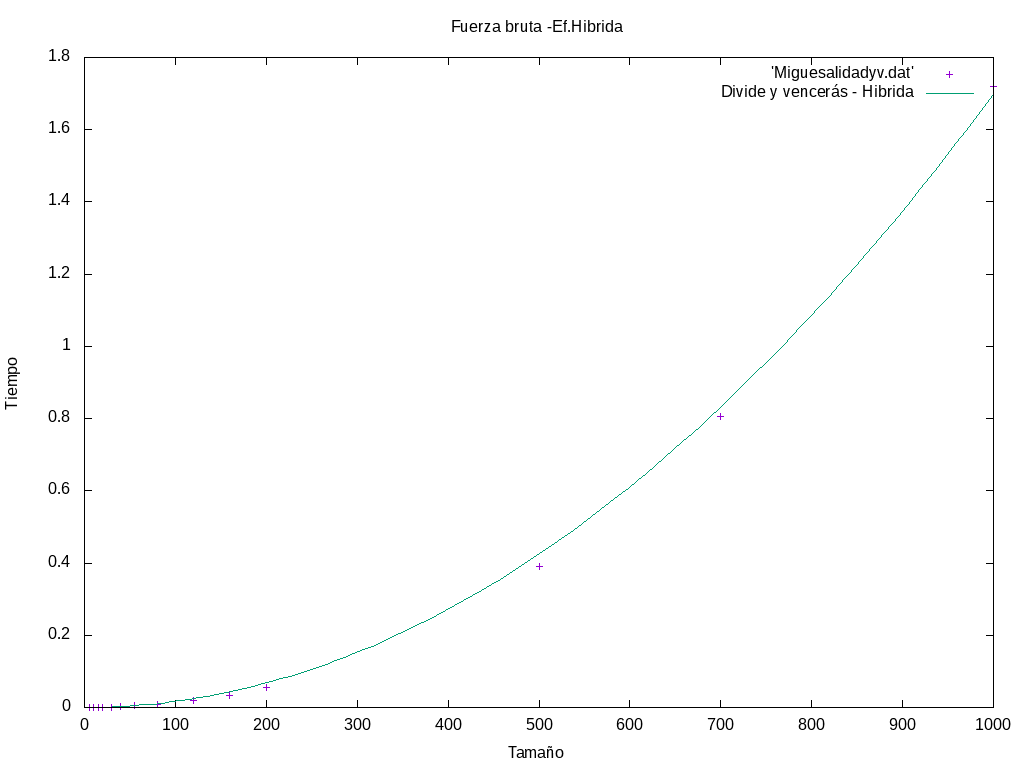
\includegraphics[width=0.7\linewidth]{../salidas-algoritmos/dyv-hibrida.png}
				\caption{	La eficiencia obtenida ha resultado ser de n cuadrado ,mejorando en un orden al de fuerza bruta.}
				\label{fig:fuerzabruta-hibrida}
			\end{figure}
\end{frame}

\section{Comparación} % Sections can be created in order to organize your presentation into discrete blocks, all sections and subsections are automatically printed in the table of contents as an overview of the talk
%------------------------------------------------
\begin{frame}
	\frametitle{Comparación}
	En esta última sección, hemos comparado los dos algoritmos que hemos desarrollado, veremos si efectivamente o no nuestra implementación utilizando un enfoque divide y vencerás obtenemos mejoras con respecto a uno de fuerza bruta.
	
\end{frame}

\begin{frame}
	\frametitle{Comparación}
	\begin{figure}[H]
		\centering
		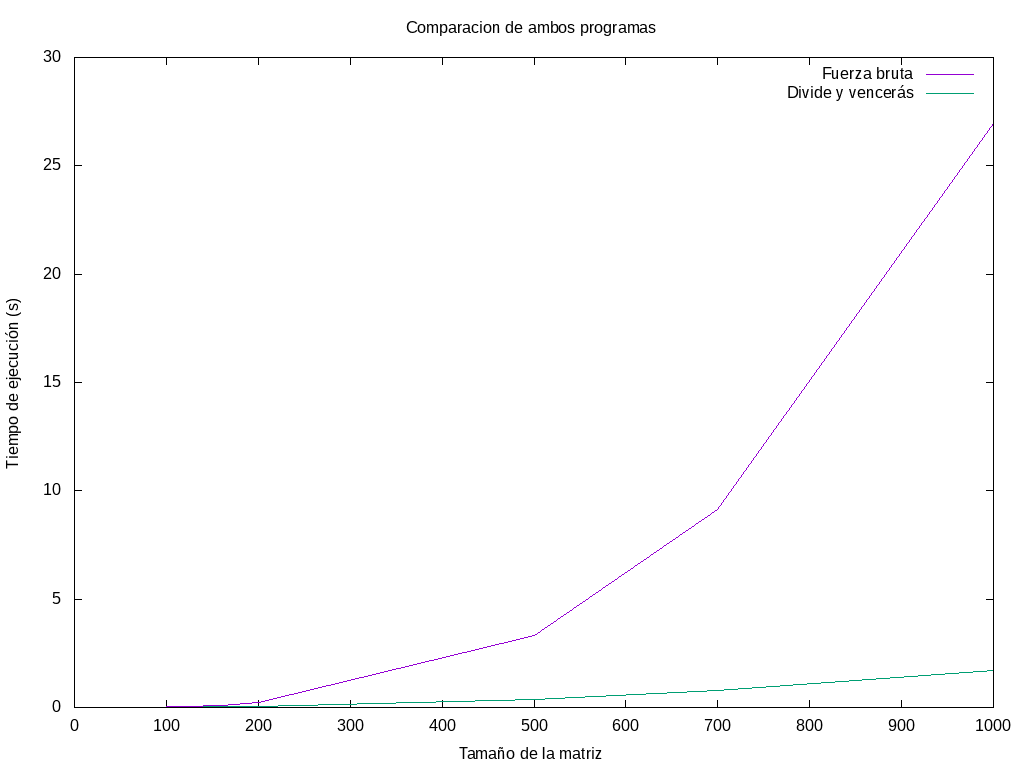
\includegraphics[width=0.7\linewidth]{../salidas-algoritmos/comparacion.png}
		\caption{Figura perteneciente a la comparación entre ambas eficiencias}
		\label{fig:fuerzabruta-hibrida}
	\end{figure}
	
\end{frame}

\begin{frame}
	\frametitle{Porcentaje de error y constantes ocultas}

\begin{center}
	\begin{tabular}{| l | c | r |}
		\hline
		\textbf{Algoritmo} & \textbf{Constante Oculta} & \textbf{Error} \\ \hline
		DyV & a0 = 1.69804e-06  & +/- 1.226e-08    (0.7218\%)\\ 
		\hline
		Fuerza bruta & a0 = 2.69052e-08 & +/- 2.352e-11    (0.0874\%)
		
	\end{tabular}
\end{center}
\end{frame}

\end{document} 
